\documentclass[11pt]{scrartcl}
\usepackage{geometry}                
\geometry{letterpaper}                   

\usepackage[english]{babel}	
\usepackage{graphicx}
\usepackage{german}
\usepackage[utf8]{inputenc} 
\usepackage{fancyhdr}
\usepackage{tabularx}
\usepackage{amssymb}
\usepackage{epstopdf}
\usepackage{natbib}
\usepackage{amssymb, amsmath}
\usepackage{float}
\usepackage{amsmath}
\usepackage{booktabs}
\usepackage{pdfpages}
\usepackage{moreverb}


\DeclareGraphicsRule{.tif}{png}{.png}{`convert #1 `dirname #1`/`basename #1 .tif`.png}

%\title{Title}
%\author{Name 1, Name 2}
%\date{date} 

\renewcommand*{\capfont}{\normalfont}
\renewcommand*{\caplabelfont}{\sffamily\bfseries}


\begin{document}



\thispagestyle{empty}

\begin{center}
\includegraphics[width=5cm]{ETHlogo.eps}

\bigskip


\bigskip


\bigskip


\LARGE{ 	Lecture with Computer Exercises:\\ }
\LARGE{ Modelling and Simulating Social Systems with MATLAB\\}

\bigskip

\bigskip

\small{Project Report}\\

\bigskip

\bigskip

\bigskip

\bigskip


\begin{tabular}{|c|}
\hline
\\
\textbf{\LARGE{Swiss Rail Network Formation with}}\\
\textbf{\LARGE{Physarum Polycephalum}}\\
\\
\hline
\end{tabular}
\bigskip

\bigskip

\bigskip

\LARGE{Lucas Böttcher \\ Simon Roth \\ Gabriela Schär}



\bigskip

\bigskip

\bigskip

\bigskip

\bigskip

\bigskip

\bigskip

\bigskip

Zurich\\
December 2012\\

\end{center}



\newpage

%%%%%%%%%%%%%%%%%%%%%%%%%%%%%%%%%%%%%%%%%%%%%%%%%

\newpage
\section*{Agreement for free-download}
\bigskip


\bigskip


\large We hereby agree to make our source code for this project freely available for download from the web pages of the SOMS chair. Furthermore, we assure that all source code is written by ourselves and is not violating any copyright restrictions.

\begin{center}

\bigskip


\bigskip


\begin{tabular}{@{}p{6cm}@{}p{6cm}@{}@{}p{6cm}@{}}
\begin{minipage}{6cm}
 \large Lucas Böttcher

\end{minipage}
& 
\begin{minipage}{6cm}
\large Simon Roth

\end{minipage}
&
\begin{minipage}{6cm}
\large Gabriela Schär

\end{minipage}
\end{tabular}
\end{center}
\newpage

%%%%%%%%%%%%%%%%%%%%%%%%%%%%%%%%%%%%%%%



% IMPORTANT
% you MUST include the ETH declaration of originality here; it is available for download on the course website or at http://www.ethz.ch/faculty/exams/plagiarism/index_EN; it can be printed as pdf and should be filled out in handwriting


%%%%%%%%%% Table of content %%%%%%%%%%%%%%%%%

\tableofcontents

\newpage

%%%%%%%%%%%%%%%%%%%%%%%%%%%%%%%%%%%%%%%



\section{Abstract}
\label{sec:abstract}

The process of continuous urbanization is noticeable in Switzerland like in the most other countries.\footnote[1]{see the autumn sunday lectures at ETH Science City (Die Stadt der Zukunft - die Zukunft der Stadt)} Besides the benefits of combining educational, medical, cultural and industrial centers in a small are, there are also some problems arising. The cities are growing, whereupon this growth in population causes an increasing use of the public transport system, which has to be adapted to the new conditions. The main goal of this project is the simulation of the Swiss rail network depending on population growth. The network is simulated with a biological inspired model based on Physarum polycephalum. This slime mold is a large single-celled amoeboid organism that forages for food sources. To maximize the searched area, it explores its environment with a relatively continuous foraging margin. It is forming different junctions and nodes to reduce the overall length of the connecting network \cite{network_tokyo}. This principle is adapted to the main railroads in Switzerland. 


\section{Individual contributions}
\begin{itemize}
  \item Lucas Böttcher
  \item Simon Roth
  \item Gabriela Schär
\end{itemize}


\section{Introduction and Motivations}
\label{sec:introduction}
Everyday thousands of commuters use the Swiss rail network to reach their workplace, school or university, mainly the same railroad is used. Seeing these facts we are going to ask, whether the actual situation of the network is the most efficient one. And related to that question, whether different connections between cities have maybe a higher performance.\\
\\
We assume, that the rail network is developed in a way that the connections between cities are the most efficient. Certain biological organisms connect their food sources in a similar way. In this project we simulate a biological organism creating its own efficient connections between the cities. This approach leads to the following main questions:

\begin{enumerate}
	\item Is the biological model a good approximation to simulate the network compared to reality?
	\item Are there any new built or destroyed connections in the network because of the future population growth?
\end{enumerate}

To answer these questions, the results of the simulations are compared with the Swiss rail network. For this comparison geodata from geodata.ethz.ch~\cite{gis_data} are used. This data are processed with \textit{ArcGis 10.1} to get the basis for the simulation.

Cities are choosen based on the numbers of inhabitants (more than 10000) in 2011 and the presence of a railaway station. Additional to these some cities with less than 10000 inhabitants are added because of actual importance for the Swiss rail network\,\cite{bfs}. ~\\
~\\
To answer the second question, we are going to manipulate parameters in Physarum network, like described  in \ref{sec:matlab}.\\
~\\
We expect that the most efficient network created by the simulation is a good approximation of the actual Swiss railroad network. We also expect that the network will not change even when the population is growing because a network changes the most at the beginning of developing. And the Swiss railroad network reaches the end of development already.




\section{Description of the Model}
\label{sec:description}

The model is inspired of the physarum polycephalum and the way this single-celled fungus searching for food. The organism have been subjected to successive rounds of evolutionary selection and have found an appropriate balance between efficiency, cost and resilience. The plasmodium contains a network of tubes, which enables chemical signals and nutrients to circulate through the organism. If some of the tubes have found food sources, this implies a positive feedback to the system. This tubes are getting thicker so the flux of nutrients increase. Other tubes which do not connect to food sources are shrinking and tend to disappear, because there is no flux available. Experiments showed two empirical rules. \textbf{1)} Tubes with no connection to a source disappear and \textbf{2)} if there are two tubes connecting the same source, the longer one disappears. This led to useful approaches to problem-solving like optimization of railroad systems or networks in general.~\\
~\\
The mathematical model is based on \textit{Physarum solver: A biologically inspired method of road-network navigation} \cite{network_model}. Figure \ref{fig:schema} shows the concept of the mathematical model. There are different nodes. The first two nodes corresponding to the food sources ($N_1$ and $N_2$) and other nodes ($N_3$, $N_4$ ... $N_j$). The junction between the node $N_i$ and $N_j$ is denoted as $M_{ij}$. In the model we connect the single nodes with circular tubes and want to measure their inner flux (Figure \ref{fig:fluidd}). Therefore the fluid dynamics prepare us with the law of Hagen-Poiseuille, which allows us to calculate the flux from the difference in pressure, the tube length and some constants. Starting from the fluid velocity in a cylindric tube \cite{kirb2010}:
\begin{figure}[H]
	\centering
	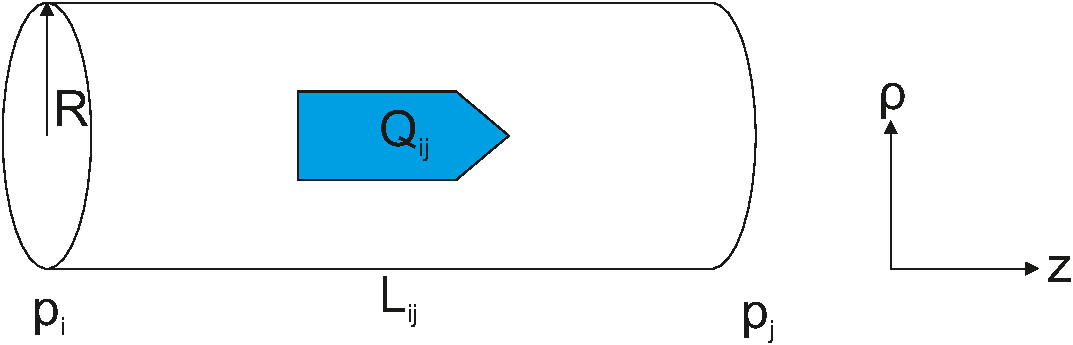
\includegraphics[width=10cm]{figures/figure2}
	\caption{Illustration of the Hagen-Poiseuille law for a circular tube, which connects the single nodes in our model.}
	\label{fig:fluidd}
\end{figure}

\begin{equation}
u(z)=-\frac{1}{4\eta}\frac{dp}{dz}(R^2-\rho^2)
\end{equation}
, where R is the radius of the cylinder and $\eta$ the viscosity. Now we can integrate that expression over a circle, and normalize to get a mean velocity:
\begin{equation}
\overline{u(z)}=-\frac{1}{4\pi\eta R^2}\frac{dp}{dz}\int_{0}^{2\pi}\int_{0}^{R}{(R^2-\rho^2)}\rho d\rho d\phi=-\frac{1}{8\eta}\frac{dp}{dz}R^2
\end{equation}
We can assume that the pressure gradient is uniform and express the mean velocity by the flux divided by its cross section:
\begin{equation}
Q_{ij}=\frac{D_{ij}}{L_{ij}}\Delta p_{ij}
\end{equation}
, where $D_{ij}=-\frac{\pi R^4}{8\eta}$ is the conductance. So we see that the Hagen-Poiseuille law is related to Ohms law, where we have a similar expression.
\begin{figure}[H]
	\centering
	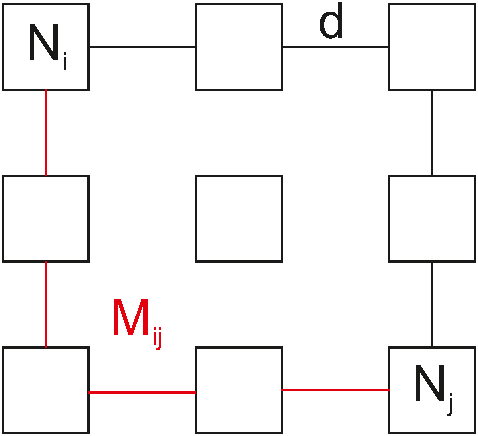
\includegraphics[width=6cm]{figures/figure1}
	\caption{\textbf{a)} Concept of the mathematical model with a source and sink node. The distance between the given nodes is a constant $d$. The centered node is not reachable. \textbf{b)} Any square represents a node with red sources, yellow transport junctions (cyan is not used) and not reachable blue terrain.}
	\label{fig:schema}
\end{figure}

The variable $Q_{ij}$ stands for the flux through the junction $M_{ij}$ from $N_i$ to $N_j$. The flux $Q_{ij}$ is given by an approximately Poiseuille flow where $p_i$ is a pressure at the node $N_i$, $L_{ij}$ is the length and $D_{ij}$ is the conductivity of the junction $M_{ij}$ :

\begin{equation}
	\label{eq:1}
	Q_{ij}=\frac{D_{ij}}{L_{ij}}\left(p_i-p_j\right)
\end{equation}

By considering Kirchhoff's law at each node, there is:

\begin{equation}
	\label{eq:2}
	\sum_{i} Q_{ij}=0 \,\,\,\, \mathrm{if} \left(j\ne 1,2\right)
\end{equation}

$N_1$ is assumed as a source node and $N_2$ as a sink and $I_0$ represent the flux from the source node and is in this model constant. It follows:

\begin{equation}
	\label{eq:3}
	\sum_{i} Q_{i1}+I_0=0, \,\,\,\, \sum_{i} Q_{i2}-I_0=0
\end{equation}

To describe the thickness of the junctions we assumed that the conductivity $D_{ij}$ changes in time according to the flux $Q_{ij}$:

\begin{equation}
	\label{eq:4}
	\frac{dD_{ij}}{dt}=f\left(\mid Q_{ij} \mid \right)-D_{ij}
\end{equation}

where $f\left(\mid Q \mid \right)$ is a increasing function with $f(0)=0$. Here $f\left(\mid Q \mid \right)$ is given by:

\begin{equation}
	\label{eq:5}
	f\left(\mid Q \mid \right)=\frac{\mid Q \mid^\gamma }{1+\mid Q \mid^\gamma}
\end{equation}

The network Poisson equation for the pressure is derived from the equations (\ref{eq:1}), (\ref{eq:2}) and (\ref{eq:3}) as followed:

\begin{equation}
	\label{eq:6}
	\sum_{i} \frac{D_{ij}}{L_{ij}}\left(p_i-p_j\right)= \begin{cases}
										-I_0 & \mathrm{for}\,\, j=1,\\
										I_0 & \mathrm{for} \,\,j=2,\\
										0 & \mathrm{otherwise}
										\end{cases}
\end{equation}

All $p_i$'s can be determined by solving the equation system (\ref{eq:6}) wenn setting $p_2=0$ as a basic pressure level. With this also each $Q_{ij}$ is obtained. They are definend bay the $D_{ij}$'s and $L_{ij}$'s  at each time step. Conductivity is closely related to the thickness of the junctions and so when a conductivity of a junction is zero, it disappears.

\section{Implementation}
\subsection{ArcGis}
\label{sec:arcgis}

To get the basis matrix for the simulation, Swiss geodata\,\cite{gis_data} are processed with \textit{ArcGis\,10.1}. Therefor the rasterdata are distinguished in different classes as in Table\,\ref{tab:class} are described.

\begin{table}[H]
	\centering
	\caption{classes of data}
		\begin{tabular}{lll}
		\toprule
		Indentification & Class & Description \\
		\midrule
		0 & Ghostland & Cells in which the slime mold isn't allowed to be\\
		& 		& (foreign coutries, lakes)\\
		1 & Freeland & Cells in which the slime mold is allowed to grow\\
		2 & Junction & Cells in which the slime mold is located, \\
		& & processed in MATLAB\\
		3 & City & Cells which represents food sources\\
		\bottomrule
	\end{tabular}
\label{tab:class}
\end{table}

All the geodata are in vector format. So all lakes and the foreign countries can be erased. It would be possible to erase more types of covering (eg. rivers, rocks) where a train can not ride. The slope is in this case also neglected. So the mountains are not considerated in the simulation. Then all the choosen cities are imported to \textit{ArcGis}. Therefor the coordinates (Y,X)\,\cite{coordinates} for each city are searched and a buffer of 2500m is layed on them. In this case no city will disapear when the vectordata gets converted to rasterdata with a cellsize of 2500m. So after converting in rasterdata with the classes above, the basis matrix is exported as ASCII-File which can now used in MATLAB as simulation surface.

To compare the simulated results with the actual Swiss rail network, different types of railroads are neglected. Therefor every tunnel and every rail road which is not in use are not showed.



\begin{figure}[H]
	\centering
	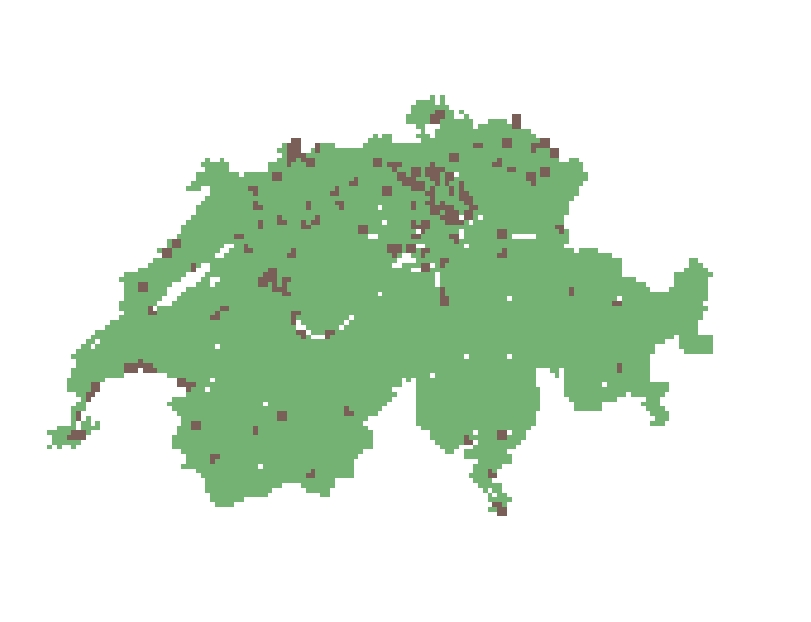
\includegraphics[width=0.7\textwidth]{figures/map_2500_cities}
	\caption{Rastardata from ArcGis with a gridsize of 2500m - white: Ghostland, green: Freeland, brown: City}
	\label{fig:map_cities}
\end{figure}


\subsection{MATLAB}
\subsubsection{Shortest Connection}
For evaluating the path length given by the Physarum simulation data, we used a program, which computes the shortest path length between two given points on the map. We use a standard algorithm \cite{gaertner2010} for implementing the function in MATLAB. In general the code uses a start coordinate from an input file, related to the map matrix A, with the defined neighborhood, i.e.:
\begin{verbatim}
function [B,short_length] = shortest_path(A,points,neigh)
\end{verbatim}
What we get by calling the function with the necessary arguments is a matrix B, which contains the given map, without citites or earlier computed ways, but with the drawn shortest path. As second output argument one can use the shortest path length as \textbf{int} value. The algorithm explained in a nutshell works can be described with the following words: After cleaning the computed matrix from cities and ways, the start entry is coded with two. As a result the matrix contains only zero elements (ghostland), ones (free land) and the start entry two. We iterate over the whole matrix entries and continue in the loop. If the entry isn't one jump to the next cell:
\begin{verbatim}
if B(k,l) ~= 1
	continue;
end
\end{verbatim}
We numerate the cells starting by two (where the next reachable cell gets the next greater natural number) and iterate with the given neighborhood:
\begin{verbatim}
if B(m,n) == step+1
B(k,l) = step+2;
iter = 1;
end
\end{verbatim}
The variable \textbf{iter} shows if there is any neighbor (=1), if not the loops stops:
\begin{verbatim}
if ~iter
break;
end
\end{verbatim}
At the end one gets a numerated way, which can be used to calculate the track length or to use a backtracking algorithm for getting the way in the matrix output matrix B. The whole program is attached to the appendix.\\
For testing the track length, computed by the Physarum simulation we used several waypoints and compared the lengths to the shortest path lengths. The outcome was that the lengths are equal. You can see one data evaluation in Figure \ref{fig:short}:
\begin{figure}[H]
	\centering
	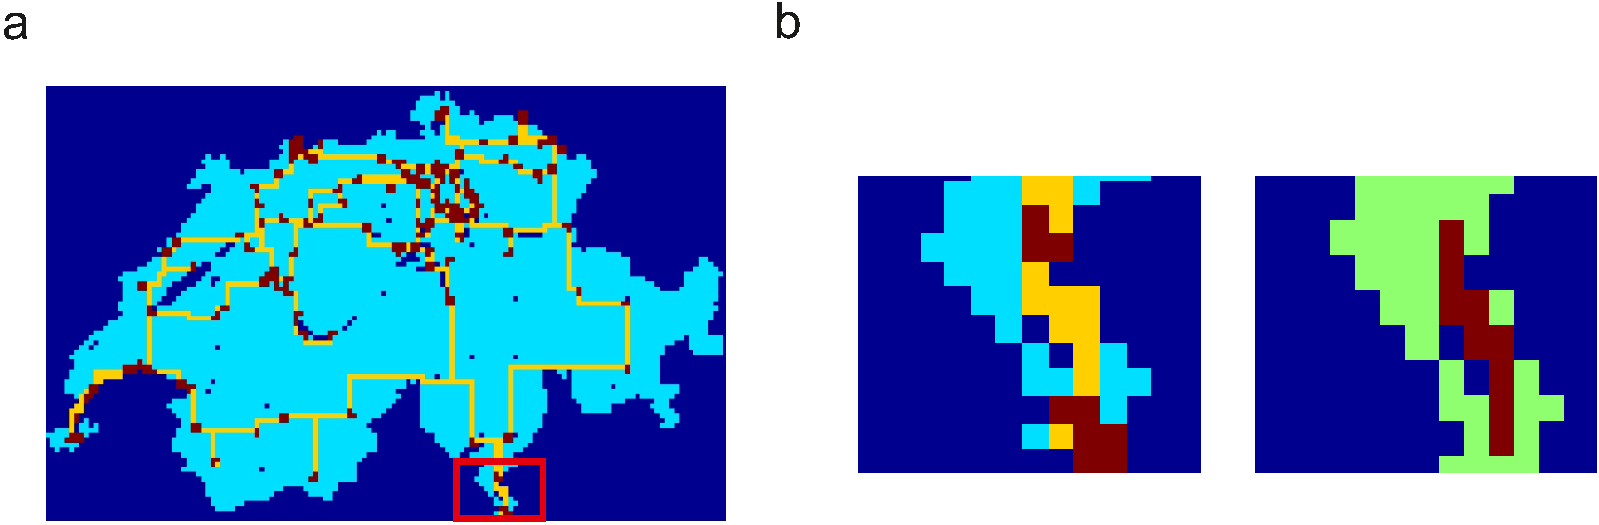
\includegraphics[width=12cm]{figures/figure3}
	\caption{\textbf{a)} Simulated track length from the Physarum simulation code. \textbf{b)} Zoomed into the red square are to see on the left hand side the Physarum simulation track length, compared to the right hand side computed shortest track length.}
	\label{fig:short}
\end{figure}
\label{sec:matlab}


\section{Simulation Results and Discussion}
\label{sec:results}
All the simulations are running with the same parameters and with a cellsize of 2500m.
\\

In Figure\,\ref{fig:path} and Figure\,\ref{fig:conductivity} are the results of the MATLAB simulation and the actual rail network showed. In this simulations are assumed that every city has an equal number of inhabitants. In Figure\,\ref{fig:path} the choosen path is ploted. Under consideration of the choosen cities that the slope is neglected is this simulated path a good approximation to the real rail network. In Figure\,\ref{fig:conductivity} is the conductivity showed that goes with the simulated path. It describes which line is used the most (eg. Bern-Solothurn-Sursee-Luzern-Zug-Zurich).

\begin{figure}[H]
	\centering
	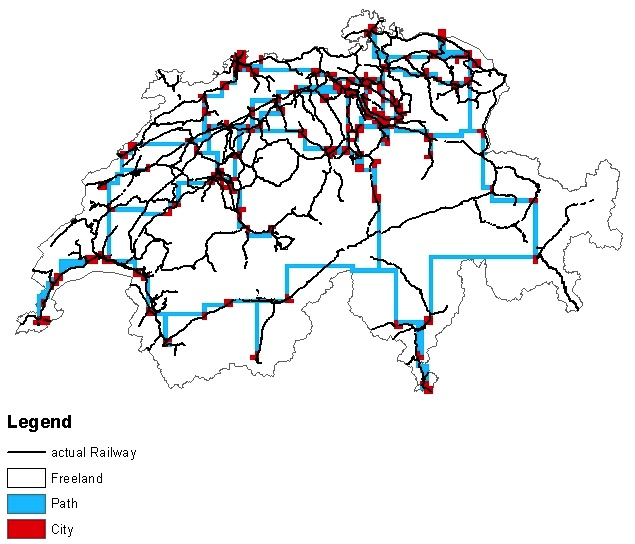
\includegraphics[width=0.7\textwidth]{figures/path_railway}
	\caption{Simulated path of Physarum polycephalum and the actual Swiss rail network}
	\label{fig:path}
\end{figure}

\begin{figure}[H]
	\centering
	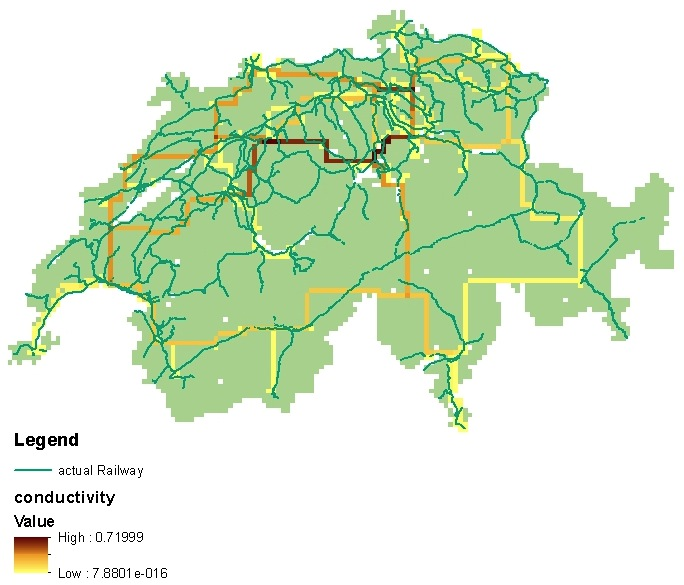
\includegraphics[width=0.7\textwidth]{figures/conductivity_railway}
	\caption{Simulated conductivity of Physarum polycephalum and the actual Swiss rail network}
	\label{fig:conductivity}
\end{figure}


\section{Summary and Outlook}
\label{sec:summary}

Summary blabla...\\
\\
There are different points to continue with this project or maybe to enlarge it in future. With more time and hardware capacity it is possible to do a lot more simulations to find the best set of parameters. Another interessting point would be to simulate the rail network with more restrictions like the slope or other surface coverings. It is also possible to simulate different scenarios of the population growth to see the consequences of the rail network developing. Another way to use the model is that the actual rail network is given and the simulation shows the utilization of the different rail lines.
Further are the international connections not considered. This could also be an additional point.



\appendix
\section{Matlab-Code}
Matlab-Code
\subsection{Shortest Path}
\begin{verbatim}
% Modeling and Simulating Social Systems with MATLAB
% http://www.soms.ethz.ch/matlab
% Author: Gabriela Schaer, Simon Roth, Lucas Boettcher 2012
% http://github.org/Trail-Formation

%PRE: A is the map with start: 2, free and end: 1, ghost 0, start and end
%coordinates from points vector and the neighborhood from neigh

%POST: Matrix B with drawn shortest path and the length (short_length)

function [B,short_length] = shortest_path(A,points,neigh)

% This function computes one shortest path and whose length between
%two points given in a 1x4 matrix, with coordinates related to the
%quadratic matrix A

% read matrix dimension
ALength1 = size(A,1);
ALength2 = size(A,2);

%initialize matrix B
B=A;

%Clear matrix B from ways and cities

for i=1:ALength1
    for j=1:ALength2
        if B(i,j)==2 || B(i,j)==3
            B(i,j)=1;
        end
    end
end

% iterate over the given points

    B(points(1),points(2)) = 2;

    % iterate over grid matrix A
            for step=1:ALength2^2
                
                % neighbor watch
                iter = 0;
                
                for k=1:ALength1
                    for l=1:ALength2
                                                    
                        if B(k,l) ~= 1
                            continue;
                        end
                        
                        % we use the linked neighborhood
                        
                        for p = 1:size( neigh, 1 )

                        m = k+neigh( p, 1 );
                        n = l+neigh( p, 2 );
                    
                        % need to respect borders
                        
                            if m >= 1 && n >= 1 && m <= ALength1 && n <= ALength2
                                
                                if B(m,n) == step+1
                                B(k,l) = step+2;
                                iter = 1;
                                end
                                
                            end
                        
                        end
                    end
                   
                end
                % if there is no other neighbor, break
                    if ~iter
                        break;
                    end
                
            end
        
       %compute the length from the marked elements in A
       short_length = B(points(3),points(4))-B(points(1),points(2));
       
       %initialize the jumping backward iteration points (for the
       %backtracking drawing of the way)
       end1=points(3);
       end2=points(4);
   for k=1:short_length
      
       for p = 1:size( neigh, 1 )

                        m = end1+neigh( p, 1 );
                        n = end2+neigh( p, 2 );
                    
                        % need to respect borders
                        
                            if m >= 1 && n >= 1 && m <= ALength1 && n <= ALength2
                                
                                if B(m,n) == B(end1,end2)-1;
                                B(end1,end2) = 2;
                                end1=m;
                                end2=n;
                                end
                                
                            end
                            continue;
       end
       
       
   end
   
    for k=1:ALength1
    for l=1:ALength2
        if B(k,l)~=2 && B(k,l)~=1 && B(k,l)~=0
            B(k,l)=1;
        end
    end
    end
end
\end{verbatim}

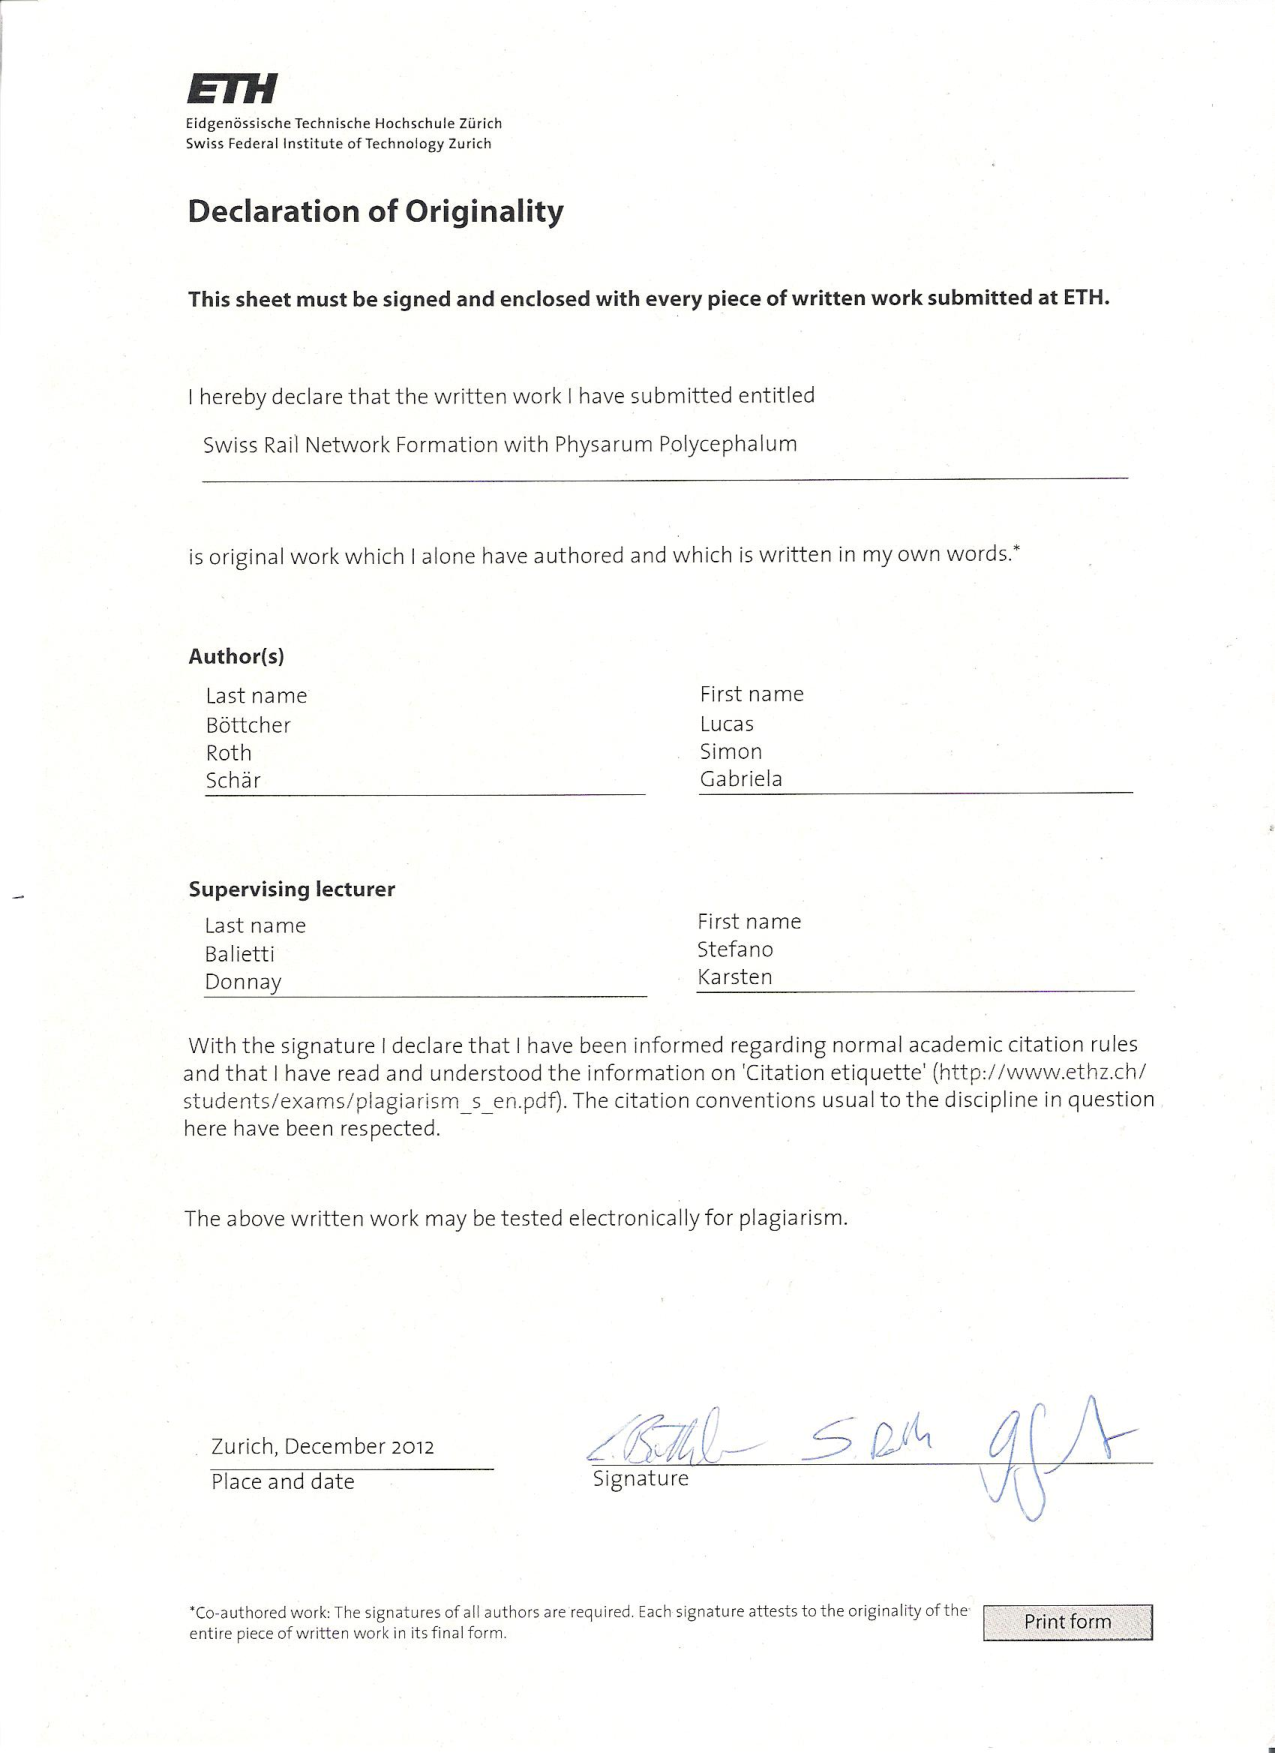
\includepdf{figures/declaration.pdf}


\bibliographystyle{plain}
\bibliography{matlabbib}






\end{document}  



 
